\documentclass{standalone}
\usepackage[T1]{fontenc}
\usepackage[utf8]{inputenc}
\usepackage{pgf,tikz}
\usepackage{setspace}
\usepackage{pgfplots}
%\pgfplotsset{compat=1.9}


\begin{document}


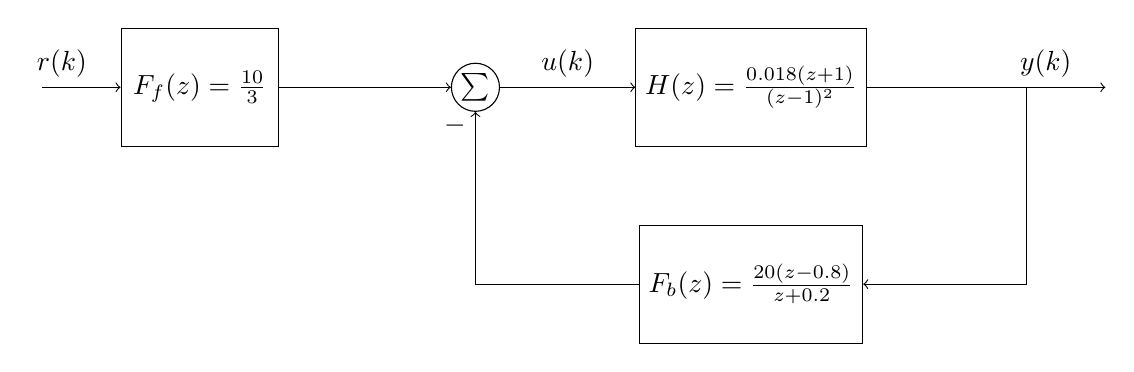
\begin{tikzpicture}[
    node distance=2cm, block/.style={rectangle, draw, minimum height=15mm, minimum width=20mm}, sumnode/.style={circle, draw, inner sep=1pt}]

  \node[coordinate] (input) {};
  \node[block, right of=input, node distance=20mm] (TR) {$F_f(z)=\frac{10}{3}$};
  \node[sumnode, right of=TR, node distance=35mm] (sum) {$\sum$};
  \node[block,right of=sum, node distance=35mm] (plant) {$H(z)=\frac{0.018(z+1)}{(z-1)^2}$};
  \node[coordinate, right of=plant, node distance=35mm] (measure) {};
  \node[coordinate, right of=measure, node distance=10mm] (output) {};
  \node[block,below of=plant, node distance=25mm] (SR) {$F_b(z)=\frac{20(z-0.8)}{z+0.2}$};

  \draw[->] (input) -- node[above, near start] {$r(k)$} (TR);
  \draw[->] (TR) -- node[above] {} (sum);
  \draw[->] (sum) -- node[above] {$u(k)$} (plant);
  \draw[->] (plant) -- node[above, near end] {$y(k)$} (output);
  \draw[->] (measure) |- (SR);
  \draw[->] (SR) -| (sum) node[left, pos=0.96] {$-$};

\end{tikzpicture}
\end{document}


